\section{Evaluation}
\label{sec:Evaluation}
This section contains the evaluation and the graphical representation of the measurements.

\subsection{Measuring the Magnetic Surface}
\label{subsec:Measuring_the_Magnetic_Surface}
The magnetic flux density was measured over a distance of about 1 m along the z-axis. The gaussmeter was zeroed at the position $z=0.6$ m. A measurement was taken every 8 cm.
\begin{figure}[H]
	\centering
	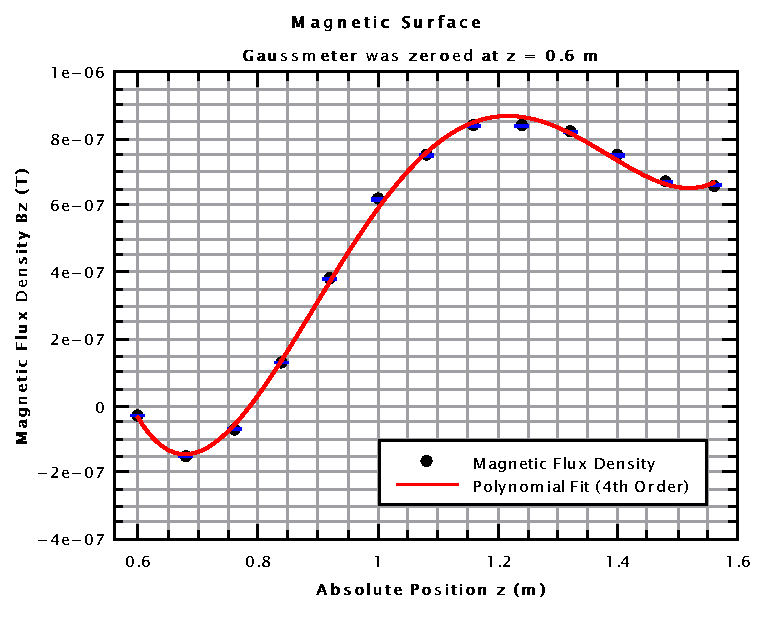
\includegraphics[scale=1]{Magnetic_Surface}
	\caption{Magnetic Surface}
	\label{fig:Magnetic_Surface}
\end{figure}
The red line in figure \ref{fig:Magnetic_Surface} shows the 4th order polynomial fit. A polynomial fit is able to represent the missing parts accurately, because the magnetic flux density can not jump. Every measuring point has the uncertainty of 0.3 \% (gaussmeter and Hall sensor) drawn in blue. Since the uncertainty is extremely small, it is almost impossible to see it. The measured values are generally very small and are therefore not used for compensation.

The resulting parameters of the 4th order polynomial fit are shown in the following table:
\begin{table}[H]
	\centering
	\renewcommand{\arraystretch}{1.3}
	\begin{tabular}{r|c|c|c|c|c}
		& \textbf{a}$_0$ & \textbf{a}$_1$ & \textbf{a}$_2$ & \textbf{a}$_3$ & \textbf{a}$_4$ \\
		\hline\hline
		\textbf{Value} & $2.031\cdot 10^{-5}$ & $-8.534\cdot 10^{-5}$ & $1.261\cdot 10^{-4}$ & $-7.747\cdot 10^{-5}$ & $1.702\cdot 10^{-5}$ \\
	\end{tabular}
	\caption{Polynomial Parameters}
	\label{tab:Polynomial_Parameters}
\end{table}
Using the polynomial parameters from the table \ref{tab:Polynomial_Parameters} above, the magnetic flux density of the surface $B_z$ at a certain position $z$ can be calculated with the following equation:
\[
B_z(z)=a_0+a_1z+a_2z^2+a_3z^3+a_4z^4
\]

\subsection{Measuring the Central Value $B_0(I)$}
\label{subsec:Measuring_the_Central_Value}
The magnetic flux density in the center of the cylindrical coil was measured in function of the current. The current ranges from 0 A to 1 A and the step size was chosen randomly.
\subsubsection{Short Cylindrical Coil}
\label{subsubsec:Short_Cylindrical_Coil}
The measured values are listed in appendix \ref{sec:Measurements}.
\begin{figure}[H]
	\centering
	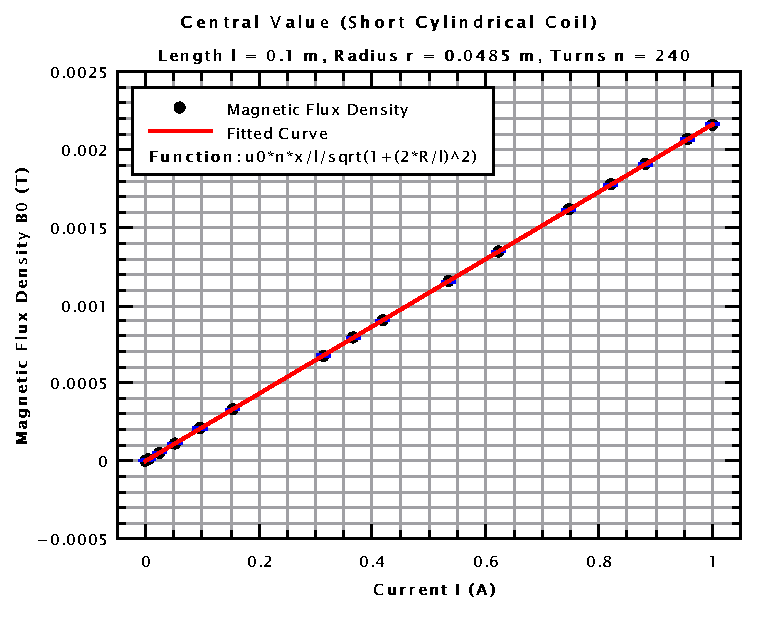
\includegraphics[scale=1]{Central_Value_Short}
	\caption{Central Value Short Cylindrical Coil}
	\label{fig:Central_Value_Short}
\end{figure}
The red fitted curve was creating by utilizing equation \ref{eq:cylindrical_coil_b0}. All parameters except the vacuum permeability $\mu_0$ were set to their according values and marked as constants. As seen in figure \ref{fig:Central_Value_Short} above, the magnetic flux density $B_0$ is proportional to the applied current $I$. The absolute error (shown in blue) of 0.3 \% is smaller than the size of a single data point and thus hard to see. The parameters of the fitted curve are listed in the following table:
\begin{table}[H]
	\centering
	\renewcommand{\arraystretch}{1.3}
	\begin{tabular}{r|l}
		& \textbf{Value} \\
		\hline\hline
		\textbf{Vacuum Permeability} $\mu_0$ & $(1.25396\pm0.00019)\cdot10^{-6}$\ $\,^\text{Vs}\!/_\text{Am}$ \\
		\textbf{Windings} $N$ & 240 (constant) \\
		\textbf{Radius} $R$ & 0.0485 m (constant) \\
		\textbf{Length} $l$ & 0.1 m (constant) \\
	\end{tabular}
	\caption{Fit Parameters (Central Value Short Cylindrical Coil)}
	\label{tab:Central_Value_Short}
\end{table}
\subsubsection{Long Cylindrical Coil}
\label{subsubsec:Long_Cylindrical_Coil}
These measurements are also listed in appendix \ref{sec:Measurements}.
\begin{figure}[H]
	\centering
	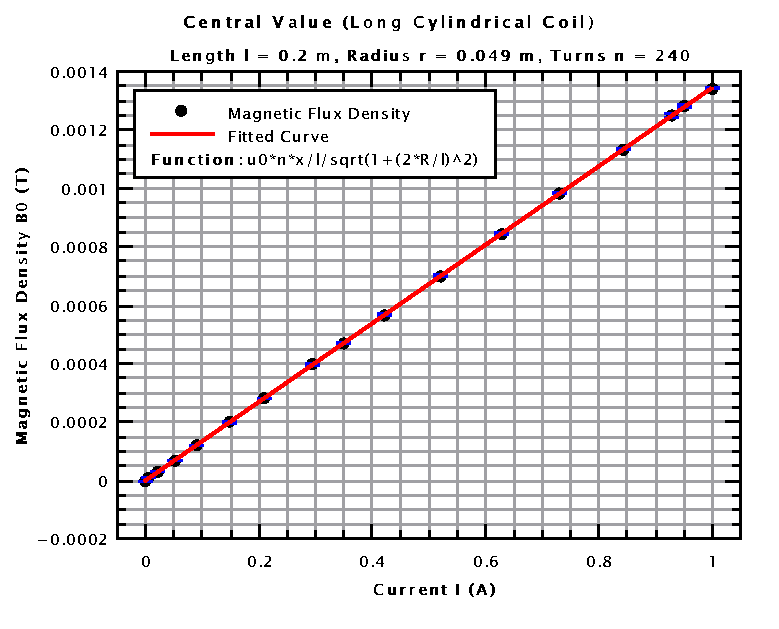
\includegraphics[scale=1]{Central_Value_Long}
	\caption{Central Value Long Cylindrical Coil}
	\label{fig:Central_Value_Long}
\end{figure}
The red fitted curve was again creating by utilizing equation \ref{eq:cylindrical_coil_b0}. The plot with the fit was created the same way as in section \ref{subsubsec:Short_Cylindrical_Coil}. The absolute error (shown in blue) of 0.3 \% is again smaller than the size of a single data point. The parameters of the fitted curve are listed in the following table:
\begin{table}[H]
	\centering
	\renewcommand{\arraystretch}{1.3}
	\begin{tabular}{r|l}
		& \textbf{Value} \\
		\hline\hline
		\textbf{Vacuum Permeability} $\mu_0$ & $(1.24853\pm0.00016)\cdot10^{-6}$\ $\,^\text{Vs}\!/_\text{Am}$ \\
		\textbf{Windings} $N$ & 240 (constant) \\
		\textbf{Radius} $R$ & 0.049 m (constant) \\
		\textbf{Length} $l$ & 0.2 m (constant) \\
	\end{tabular}
	\caption{Fit Parameters (Central Value Long Cylindrical Coil)}
	\label{tab:Central_Value_Long}
\end{table}
\newpage
\subsection{Measuring the Field Pattern $B_z(z)$}
\label{subsec:Measuring_the_Field_Pattern}
To measure the field pattern, the current was set to about 1 A. Then the cylindrical coil was moved along the z-axis and measurements were taken in dependence of how fast the magnetic flux density changed.
\subsubsection{Short Cylindrical Coil}
\label{subsubsec:Short_Cylindrical_Coil_Field}
\begin{figure}[H]
	\centering
	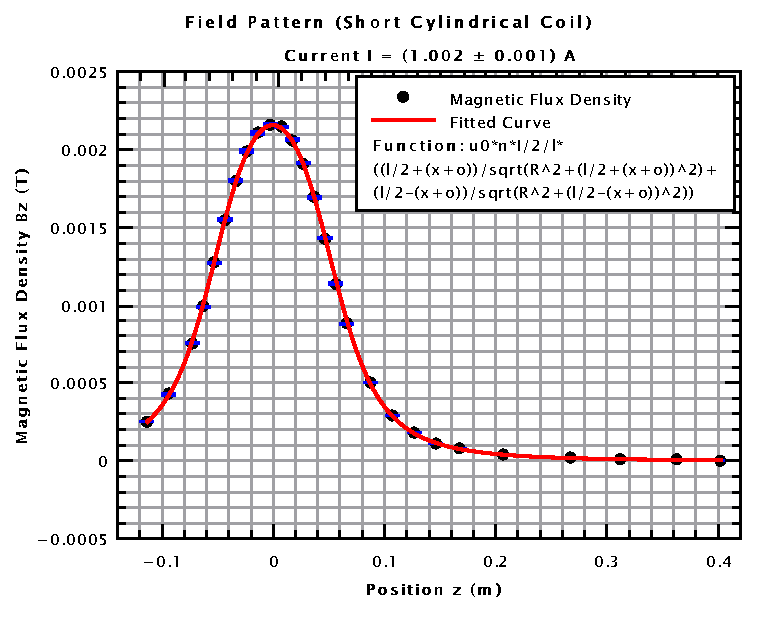
\includegraphics[scale=1]{Field_Pattern_Short}
	\caption{Field Pattern Short Cylindrical Coil}
	\label{fig:Field_Pattern_Short}
\end{figure}
The fitted curve was created by using equation \ref{eq:cylindrical_coil_bz}. All parameter except the vacuum permeability $\mu_0$ and an offset $o$ were defined and set as constants. The offset $o$ is essential because the position of the Hall sensor is not exactly known. Furthermore, the ruler scale used to determine the $z$ values has an uncertainty of 1 mm. By using an offset, the fit is able to correct for those errors. The absolute error is shown in blue. The following parameter were obtained:
\begin{table}[H]
	\centering
	\renewcommand{\arraystretch}{1.3}
	\begin{tabular}{r|l}
		& \textbf{Value} \\
		\hline\hline
		\textbf{Vacuum Permeability} $\mu_0$ & $(1.25017\pm0.00063)\cdot10^{-6}$\ $\,^\text{Vs}\!/_\text{Am}$ \\
		\textbf{Offset} $o$ & $(0.26\pm0.04)$ mm \\
		\textbf{Windings} $N$ & 240 (constant) \\
		\textbf{Current} $I$ & 1.002 A (constant) \\
		\textbf{Radius} $R$ & 0.0485 m (constant) \\
		\textbf{Length} $l$ & 0.1 m (constant) \\
	\end{tabular}
	\caption{Fit Parameters (Field Pattern Short Cylindrical Coil)}
	\label{tab:Field_Pattern_Short}
\end{table}
\subsubsection{Long Cylindrical Coil}
\label{subsubsec:Long_Cylindrical_Coil_Field}
All measured values are listed in appendix \ref{sec:Measurements}.
\begin{figure}[H]
	\centering
	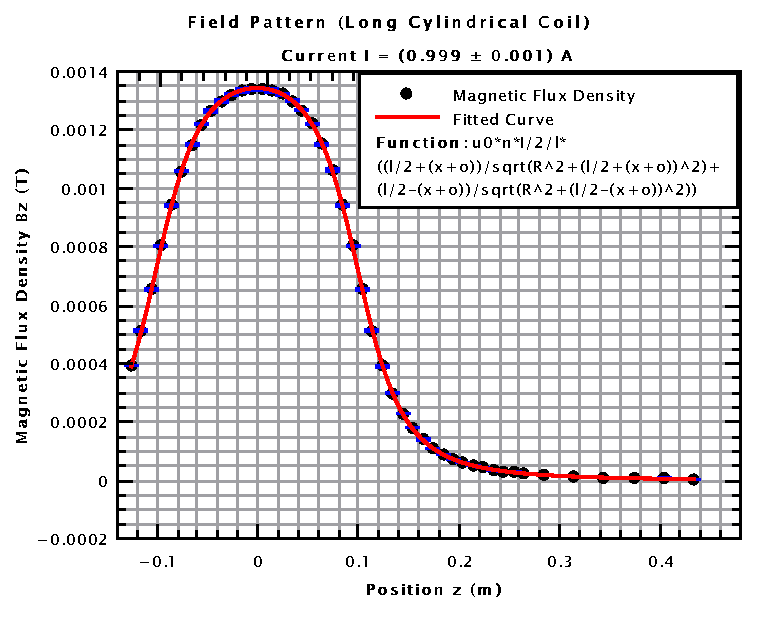
\includegraphics[scale=1]{Field_Pattern_Long}
	\caption{Field Pattern Long Cylindrical Coil}
	\label{fig:Field_Pattern_Long}
\end{figure}
The red fitted curve was again creating by utilizing equation \ref{eq:cylindrical_coil_bz}. The plot with the fit was created the same way as in section \ref{subsubsec:Short_Cylindrical_Coil_Field}. Since the uncertainty of the gaussmeter (combined with the Hall sensor) is so small, it is hard to see the error (shown in blue). The following parameters were obtained from the fit:
\begin{table}[H]
	\centering
	\renewcommand{\arraystretch}{1.3}
	\begin{tabular}{r|l}
		& \textbf{Value} \\
		\hline\hline
		\textbf{Vacuum Permeability} $\mu_0$ & $(1.24867\pm0.00036)\cdot10^{-6}$\ $\,^\text{Vs}\!/_\text{Am}$ \\
		\textbf{Offset} $o$ & $(0.97\pm0.03)$ mm \\
		\textbf{Windings} $N$ & 240 (constant) \\
		\textbf{Current} $I$ & 0.999 A (constant) \\
		\textbf{Radius} $R$ & 0.049 m (constant) \\
		\textbf{Length} $l$ & 0.2 m (constant) \\
	\end{tabular}
	\caption{Fit Parameters (Field Pattern Long Cylindrical Coil)}
	\label{tab:Field_Pattern_Long}
\end{table}
